%%%%%%%%%%%%%%%%%%%%%%%%%%%%%%%%%%%%%%%%%%%%%%%%%%%%%%%%%%%%%%%%%%%%%%%%%%%%%%%%
% Template for ASPLOS papers.
%
% History:
% 
% ASPLOS originally used jpaper.cls for submission but required acmart.cls for the
% final camera-ready version. To avoid a change in format, starting ASPLOS 2024 Fall 
% cycle, both the submission and the camera-ready versions started using acmart.cls.
%
%%%%%%%%%%%%%%%%%%%%%%%%%%%%%%%%%%%%%%%%%%%%%%%%%%%%%%%%%%%%%%%%%%%%%%%%%%%%%%%%%%

% use the base acmart.cls version 1.92
% use the sigplan proceeding template with the default 10 pt fonts
% nonacm option removes ACM related text in the submission. 
\documentclass[nonacm,sigplan]{acmart}

% enable page numbers
\settopmatter{printfolios=true}

% make references clickable 
\usepackage[]{hyperref}
\usepackage{xcolor}
\usepackage{url}
\usepackage{soul}
\usepackage{listings}
\usepackage{courier}
\usepackage{multirow}
\usepackage{array}
\usepackage{enumitem}
\usepackage{booktabs}
\usepackage{ragged2e} % For text alignment
\usepackage{geometry} % For page layout
\usepackage{siunitx}
\newcommand{\note}[1]{{\bf{\color{red}*** {#1} ***}}}


\begin{document}

\title{Evaluation of Big Data Analytics Frameworks Using Extended Heaps over Fast Remote Storage Systems}
\subtitle{\large{Undergraduate Thesis}}

\author{Theodoros Pontzouktzidis}
\affiliation{%
  \institution{Department of Computer Science, University of Crete, Greece}
  \country{Author}
  }
\email{csd4336@csd.uoc.gr}
\authornote{Thesis advised by Angelos Bilas, Professor Department of Computer Science, University of Crete, Greece}

\begin{abstract}
Today big data analytics frameworks running on managed runtimes, such as Java
Virtual Machines (JVM) are extensively used in data centers for analyzing large
datasets. Existing research has explored extending the managed heap using fast
storage devices (e.g., NVMe SSDs) and remote memory. However, a comprehensive
comparison of these techniques is lacking, underscoring the need for detailed
studies evaluating their performance, and reliability.

In our comparative analysis, we investigate strategies for optimizing block
storage access and sizing, focusing on local NVMe SSDs versus remote storage
devices and DRAM. We break down and examine the latencies of local and remote
storage systems, including SPDK NVMe over Fabrics (NVMe-oF) and Network Block
Device (NBD). Using TeraHeap, which extends JVM capabilities by utilizing a
second heap on a storage device, we compare its performance with local and 
remote systems. Our evaluation, conducted using 13 widely-used
applications in two real-world big data frameworks, Spark and Giraph,
demonstrates that remote NVMe and remote Ram-disk can match the performance of local NVMe.

\end{abstract}


\keywords {large analytics datasets, large managed heaps, fast storage devices, remote storage, systems performance}


\maketitle % should come after the abstract
\pagestyle{plain} % should come right after \maketitle

\section{Introduction}
%% Demand for more memory
Big data analytics frameworks running on managed runtimes, such as Java virtual
machines (JVM) are widely deployed in data-centers to perform data analysis over
large amount of datasets. The amount of data increases with high rate but DRAM
capacity in a single server scales slower than data growth. Existing approaches
study the extension of the managed heap over fast storage devices (e.g., NVMe
SSDs) and remote memory.

%Today, cloud infrastructures running data-intensive applications encounter
%numerous challenges in transferring data to-from block storage devices. 
%With the
%escalating demands of big data frameworks, the insufficiency of DRAM in scaling
%to such magnitudes becomes apparent. Additionally, traditional approaches to
%accessing local storage devices struggle to match the pace of data processing,
%thereby becoming an overhead. Consequently, the rapid expansion of data
%necessitates a swift and efficient mechanism for data movement to storage
%devices.

Related work that extend the managed heap beyond local DRAM either uses local storage devices~\cite{XXX} or remote memory~\cite{XXXX}. However, current
research lacks a comprehensive comparison of these techniques. None of the
existing work adequately addresses the pros and cons of each approach or
explains why one might be preferable over the others. This gap highlights a need
for detailed evaluative studies that assess the performance, and reliability of
each heap extension implementation method.

%categorization of how you can have an extended heap approaches like using a extended heap over local storage device or over remote storage device or remote DRAM memory exist...

%However, non of existing work provide a comparison between the techniques on what are the pros and cons and why they are better from one another...

In this comparative analysis, we delve into possible strategies for achieving
faster and more efficient block storage accessing while ensuring an appropriate
size of the block storage. The first aspect of our investigation centers on
comparing local storage devices, exemplified by NVMe SSDs, against remote
storage devices and remote DRAM memory. NVMe SSDs, offer rapid data access and
reliability. However, the efficiency of local storage devices in comparison to
remote options remains a question mark and forms the core of our study. Remote
DRAM memory, despite its remote positioning, may offer lower latency compared to
remote storage devices due to its faster access times. However, its capacity is
typically more constrained than storage devices. It's crucial to note the role
of technological advancements such as SPDK NVMe over Fabrics (NVMe-oF) in
mitigating latency concerns. SPDK NVMe-oF holds promise in reducing device
latency, offering a potential solution to bridge the performance gap between
different storage modalities. 

By employing micro-benchmarks we try to discern the inherent trade-offs. This
evaluation is crucial for comprehensively understanding the landscape of storage
solutions and their applicability in real-world scenarios. To assess the
performance of block device setups, we leverage TeraHeap. TeraHeap extends the
capabilities of the JVM and utilizes a second heap stored on a storage device.
This approach allows for a meticulous evaluation of storage solutions, providing
nuanced insights into their performance characteristics. Our evaluation process,
empowered by TeraHeap, furnishes high-level results that offer valuable insights
into the comparative advantages and limitations of each storage solution.

The selection among these options requires careful consideration of factors such
as workload requirements and infrastructure configurations. The insights
acquired by this study will play a pivotal role in informing decision-making
processes related to resource allocation and system design, thereby contributing
to the ongoing discourse on efficient data management in contemporary computing
environments.

%\subsection{Key Contribution}

\section{Background}

In this section, we discuss the design of state-of-the art systems that provide
access to remote memory and storage. Specifically, in our study we use Network
Block Device (NBD), NVMe over Fabrics (NVMe-oF), and the Storage Performance
Development Kit (SPDK).
\subsection{Network Block Device (NBD)}
 Network Block Device (NBD) is a network protocol that can be used to export a block device from a server where the block device resides to a client. There are multiple NBD implementations
 some of them are :
 \begin{itemize}
 \item  \textbf{nbdkit} is a multi-threaded NBD server with a plugin architecture.
 \item  \textbf{libnbd} is a library to aid in writing NBD clients
 \item  \textbf{qemu} contains an \textbf{embedded NBD server}, \textbf{an embedded NBD client}, and \textbf{a standalone NBD server} (qemu-nbd). They maintain a status document of their NBD implementation.
 \item  A \textbf{GEOM gate-based client implementation for FreeBSD} exists. It has not seen any updates since 2018, and only implements the client side (any server should run on FreeBSD unmodified, however).
 \item  A \textbf{Windows} client implementation exists as part of the RBD implementation of Ceph for Windows.
 \item  \textbf{lwNBD} is a NBD server library, targetting bare metal or OS embedded system. It has a plugin architecture.
 \end{itemize}
 We will focus on the Network Block Device (TCP version). We use the TCP version to investigate the overheads added by the TCP protocol stack and compare it with other mechanisms for exporting block devices over the network.With this implementation compiled in the kernel we can use 2 drivers-modules the nbd-client and the nbd-server Figure \ref{fig:nbd_path} shows an overview of a NBD system.
 \begin{figure}[h]
    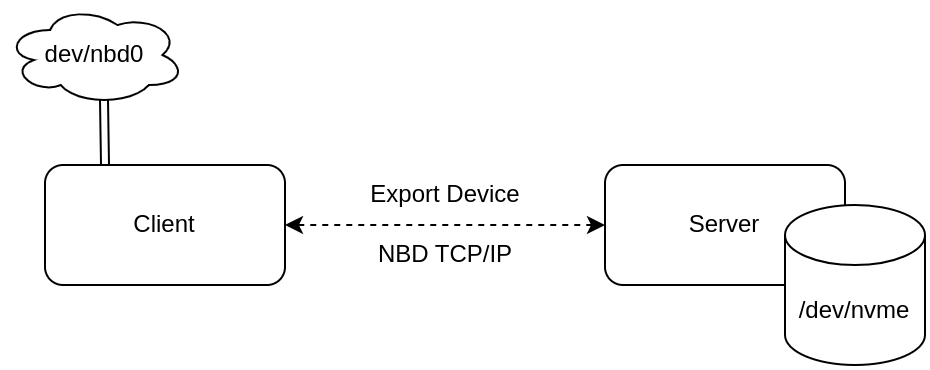
\includegraphics[scale=0.22]{figures/nbd-path.png}\\
    \caption{Overview of an NBD system.}
    \label{fig:nbd_path}
  \end{figure}
\par The nbd-client usually resides in the OS kernel and exposes a block device interface to the rest of the kernel, so that it may appear as an ordinary, directly-attached storage device. The client passes the block requests to the NBD driver where they are encapsulated as NBD network messages and sent to the server via TCP. Finally the User-Space server upon receiving the NBD request issues standard I/O to the relevant block device and then responds Figure \ref{fig:nbd_path2} shows a more in depth I/O path using NBD TCP Version. 
\begin{figure}[h]
    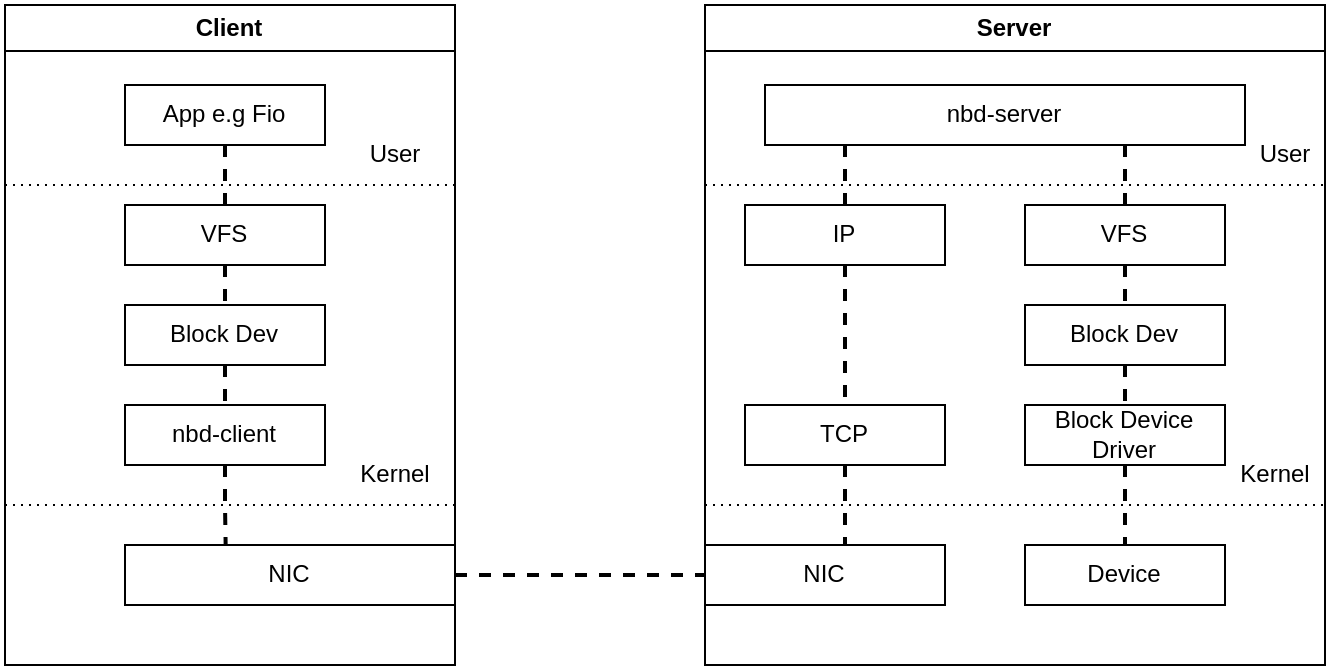
\includegraphics[scale=0.18]{figures/nbd-path2.png}\\
    \caption{I/O Path of NBD system.}
    \label{fig:nbd_path2}
  \end{figure}

\subsection{NVMe over Fabrics (NVMe-oF)}
NVMe over Fabrics (NVMe-oF) is a protocol specification designed for connecting
hosts to storage systems over a network using the NVMe protocol. It enables the
transfer of data between a host computer and a target solid-state storage device
or system through network communication. This protocol utilizes NVMe
message-based commands to facilitate data transfers, supporting various
networking technologies such as Ethernet, Fibre Channel (FC), and InfiniBand.

\subsection{Storage Performance Development Kit (SPDK)}
The Storage Performance Development Kit (SPDK) is a versatile toolkit tailored
for crafting high-performance, scalable storage applications in user-mode
environments. Its architecture revolves around several core principles aimed at
optimizing performance like User-Space Drivers, Polling Mechanism and lockless
I/O handling. At its foundation, SPDK features a user-space, asynchronous NVMe
driver designed for zero-copy, highly parallel access to SSDs. This driver,
presented as a C library with a simple public header, facilitates seamless
integration for developers. Additionally, SPDK offers a user-space block stack
library mirroring OS functionalities, including storage device interface
unification, queue management for resource constraints, and logical volume
administration. SPDK extends its capabilities with NVMe-oF, iSCSI, and vhost
servers built atop these foundational components. 

\par SPDK operates entirely in user space, bypassing the kernel entirely for I/O operations. By eliminating the overhead of kernel context switches and system calls, SPDK can achieve significantly higher performance and lower latency compared to traditional storage solutions that rely on kernel-level operations. Memory management in SPDK is highly optimized, utilizing techniques such as large memory buffers, memory pooling, and zero-copy operations. Large memory buffers are allocated upfront, often using huge pages, to ensure contiguous memory allocation and reduce fragmentation. Memory pooling minimizes the overhead of dynamic memory allocation and deallocation, while zero-copy operations eliminate unnecessary data copies, further enhancing performance. Integration with the Data Plane Development Kit (DPDK) enhances SPDK's performance by leveraging DPDK's efficient packet processing capabilities for networked storage solutions. This integration enables SPDK to handle network I/O with minimal overhead, ensuring high throughput and low latency for storage applications deployed in networked environments. SPDK's support for NVMe-oF extends the NVMe protocol over fabrics, allowing remote access to NVMe storage devices with minimal overhead. This involves sophisticated handling of NVMe commands and data over high-speed networks, optimizing performance and scalability for distributed storage solutions.
\begin{figure}[H]
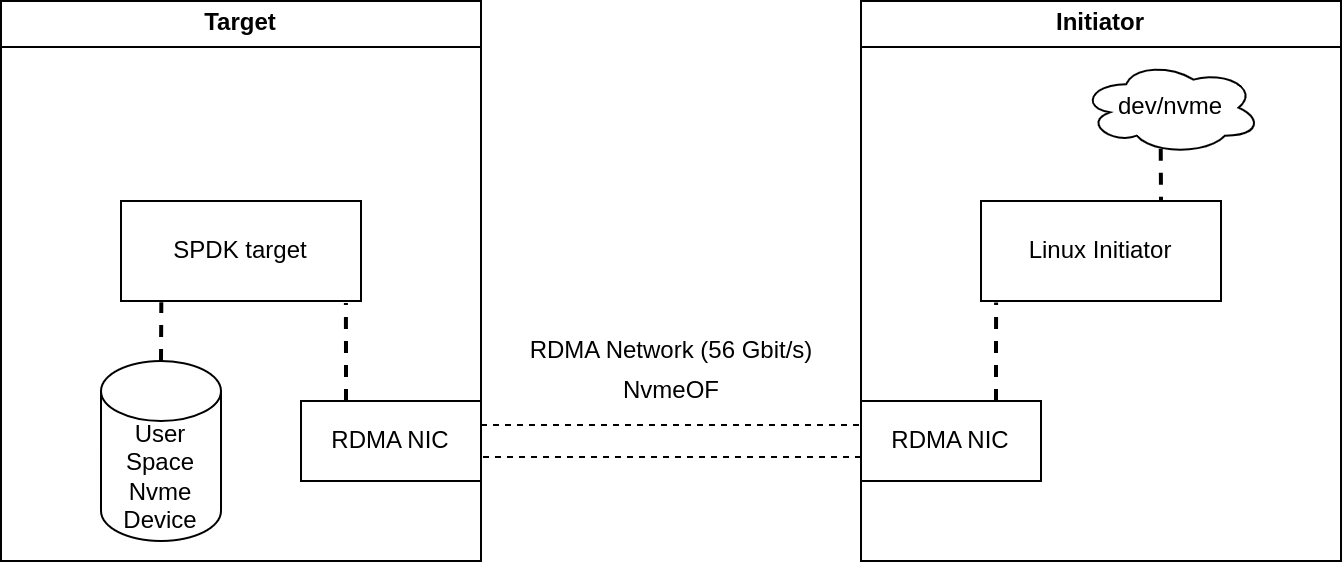
\includegraphics[scale=0.18]{figures/spdk-target.png}\\
\caption{Overview of SPDK NvmeOF Target-Initiator system.}
\label{fig:spdk}
\end{figure}
\par Figure \ref{fig:spdk} Shows the overview of the SPDK NVMe-oF Target-Initiator system. The process begins with the target unbinding traditional kernel drivers associated with the block device and binding them with SPDK's user-space drivers. This step grants SPDK exclusive control over the block device, enabling optimized I/O handling and performance. Subsequently, the block device, now under the control of SPDK in user space, is exported to the network using the NVMe-oF protocol specification, facilitated by RDMA. RDMA plays a pivotal role in enabling high-speed, low-latency data transfers over the network, allowing direct access to remote system memory without CPU involvement. This exportation process ensures efficient data transmission between the NVMe target and initiator. Additionally, SPDK supports kernel initiators, allowing traditional kernel-based applications to connect to SPDK NVMe-oF targets. Through this mechanism, kernel initiators can access the SPDK-exported block device over the network using standard device nodes such as /dev/nvme.
\section{Experimental Methodology}
With our evaluation we try to answer: 

1. Can remote storage options keep up with local ones in big data analytic
    frameworks.

2. How does data granularity affect remote options (e.g. 512B and 4KB).

3. what are the overheads presented with these options.

%\note{jk: Make the questions more specific. For example, add a question about
%granularity (e.g. 512b and 4KB). So, think carefully what was the evaluation
%about and write specific questions. Do not care if they are too much, we are
%going to reduce/merge them.}
\vspace{1em}

For the evaluation we use two servers with Intel Xeon E5-2630 32 Cores @ 2.4
GHz. Each server uses 256GB of DDR4 DRAM divided on two NUMA nodes, each with 16
threads. For storage we use Samsung 970 EVO Plus 2 TB PCIe Gen 3.0 x4 NVMe SSD.
Each server is equipped with Mellanox Technologies ConnectX-3 Network controller
MT27500 with fibre ports compliant with the InfiniBand Architecture
Specification . The servers run CentOS version 7.9 with Linux kernel version is
5.4.267. Table \ref{tab:serv_specs} shows the server specifications.
\begin{table}[H]
\resizebox{8.5cm}{1cm}{%
\begin{tabular}{cccccc}
\textbf{ID} & \textbf{CPU}                                                                      & \textbf{DRAM}                                        & \textbf{Device}                                                                       & \textbf{NIC}                                                                       & \textbf{Kernel} \\ \hline
Server 1    & \begin{tabular}[c]{@{}c@{}}Intel Xeon E5-2630\\  32 Cores @ 2.4 GHz.\end{tabular} & \begin{tabular}[c]{@{}c@{}}256GB\\ DDR4\end{tabular} & \begin{tabular}[c]{@{}c@{}}Samsung 970 EVO \\ Plus 2 TB PCIe \\ NVMe SSD\end{tabular} & \begin{tabular}[c]{@{}c@{}}Mellanox Technologies \\ ConnectX-3 MT2750\end{tabular} & 5.4.267         \\ \hline
Server 1    & \begin{tabular}[c]{@{}c@{}}Intel Xeon E5-2630\\  32 Cores @ 2.4 GHz.\end{tabular} & \begin{tabular}[c]{@{}c@{}}256GB\\ DDR4\end{tabular} & \begin{tabular}[c]{@{}c@{}}Samsung 970 EVO \\ Plus 2 TB PCIe \\ NVMe SSD\end{tabular} & \begin{tabular}[c]{@{}c@{}}Mellanox Technologies \\ ConnectX-3 MT2750\end{tabular} & 5.4.267        
\end{tabular}
}
\caption{Server specifications table.}
\label{tab:serv_specs}
\end{table}

\par\textbf{Flexible I/O (FIO) Tester.}
FIO is a widely used open-source tool in the Linux ecosystem for benchmarking
and testing various I/O (input/output) workloads on storage devices. FIO
provides detailed output reports, including metrics such as throughput, IOPS
(input/output operations per second), latency, and CPU utilization. We use FIO to measure latency of each of the device setups shown in Table \ref{tab:storage_configurations}. 

\begin{table}[h!]
\centering
\resizebox{8.8cm}{2.4cm}{%
\begin{tabular}{>{\RaggedRight}p{5cm} >{\RaggedRight\arraybackslash}p{9cm}}
\toprule
\textbf{Configuration} & \textbf{Description} \\
\midrule
Local NVMe drive & Local Non-Volatile Memory Express (NVMe) storage drive. \\
\addlinespace[1em]
Local Ram-disk & Storage using a portion of system RAM as a high-speed drive. \\
\addlinespace[1em]
Network Block Device (NBD) with NVMe & Network Block Device configured to use an NVMe drive over the network. \\
\addlinespace[1em]
Network Block Device (NBD) with Ram-disk & Network Block Device configured to use a RAM-disk over the network. \\
\addlinespace[1em]
Local NVMe drive with SPDK User-Space drivers & Local NVMe drive managed with Storage Performance Development Kit (SPDK) user-space drivers. \\
\addlinespace[1em]
Local Ram-disk with SPDK User-Space drivers & Local RAM-disk managed with SPDK user-space drivers. \\
\addlinespace[1em]
NVMe-oF NVMe with SPDK User-Space drivers & NVMe over Fabrics (NVMe-oF) using NVMe drives managed with SPDK user-space drivers. \\
\addlinespace[1em]
NVMe-oF Ram-disk with SPDK User-Space drivers & NVMe-oF using RAM-disk managed with SPDK user-space drivers. \\
\bottomrule
\end{tabular}
}
\caption{Storage device setups.}
\label{tab:storage_configurations}
\end{table}

\par\textbf{Netperf.} 
Netperf is a benchmarking tool used to measure the performance of networking
systems. It's designed to provide a standardized method for measuring networking
performance between two systems. Netperf allows users to test various aspects of
networking performance, such as throughput, latency, and jitter, across
different network protocols like TCP (Transmission Control Protocol) and UDP
(User Datagram Protocol). We will use Netperf to measure end-to-end latency of
TCP (Transmission Control Protocol) To better understand the latency of systems
like Network Block Device (NBD) which uses TCP to export the block device to the
network.

\par\textbf{TeraHeap.} Teraheap is a system that eliminates S/D overhead and expensive GC scans for a
large portion of the objects in big data frameworks. TeraHeap enhances the
managed runtime environment, particularly the Java Virtual Machine (JVM). It
introduces a supplementary heap, designed for high-capacity storage, alongside
the primary heap. This secondary heap utilizes fast storage and allows direct
access to objects without the need for serialization or deserialization.
Additionally, TeraHeap minimizes the garbage collection overhead by preventing
the garbage collector from scanning the secondary heap. It takes advantage of
frameworks' capability to designate certain objects for off-heap allocation and
provides them with a hint-based method for relocating these objects to the
secondary heap. We will use Teraheap as a Real world system. We configure Teraheap to apply the supplementary heap to local and remote block devices and compare the performances of each block device system.
\par\textbf{ib\_read\_lat.} ib\_read\_lat is a benchmarking tool specifically for measuring InfiniBand (IB) latency. It evaluates the time taken for data to be transferred and received between InfiniBand endpoints. We will use it to measure the latency of transferring data between two Mellanox Technologies ConnectX-3 MT2750 network cards using the IB port.
\par\textbf{Workloads and Execution time breakdown.} We employ eight memory-intensive tasks from Spark-Bench and five LDBC Graphalytics suites for Giraph, generating datasets accordingly. Each experiment is run five times, and the average end-to-end execution time is recorded. Time breakdown includes 'other' time, S/D plus I/O time, minor GC time, and major GC time. 'Other' time covers mutator threads, potentially including I/O wait. The profiler operates with minimal overhead. We configure TeraHeap to allocate the first heap (H1) on DRAM and the second heap (H2) over a file in Local or Remote block device via memory-mapped I/O (mmio) we also limmit DRAM and H1 to a fixed size to create pressure and more I/O to H2. Table \ref{tab:workloads} shows the DRAM and H1 size in each workload, in Spark and Giraph, accordingly.
\begin{table}[h]
\centering
\resizebox{8.2cm}{2.4cm}{%
\begin{tabular}{|c|l|r|r|}
\hline
\multicolumn{1}{|l|}{\textbf{Frameworks}} & \textbf{Benchmarks} & \multicolumn{1}{c|}{\textbf{TOTAL DRAM (GB)}} & \multicolumn{1}{c|}{\textbf{H1 (GB)}} \\ \hline
\multirow{8}{*}{\rotatebox[origin=c]{90}{\textbf{Spark}}} & Pagerank & 80 & 64 \\ \cline{2-4} 
 & Connected Components & 84 & 68 \\ \cline{2-4} 
 & Linear Regression & 54 & 27 \\ \cline{2-4} 
 & Logistic Regression & 54 & 27 \\ \cline{2-4} 
 & Triangle Counts & 80 & 64 \\ \cline{2-4} 
 & Shortest Path & 58 & 42 \\ \cline{2-4} 
 & SVDPlusPlus & 40 & 24 \\ \cline{2-4} 
 & SVM & 48 & 32 \\ \hline
\multirow{5}{*}{\rotatebox[origin=c]{90}{\textbf{Giraph}}} & PageRank & 85 & 50 \\ \cline{2-4} 
 & CDLP & 85 & 60 \\ \cline{2-4} 
 & WCC & 85 & 60 \\ \cline{2-4} 
 & BFS & 65 & 35 \\ \cline{2-4} 
 & SSSP & 90 & 50 \\ \hline
\end{tabular}%
}
\caption{Teraheap workload configuration table.}
\label{tab:workloads}
\end{table}

\section{Evaluation}
\subsection{Storage systems latency.}
We use FIO to measure how much latency each different storage system adds.
Figure \ref{fig:fio_512} shows the latency with 512 bytes request size
of each storage system.

\begin{figure}[H]
  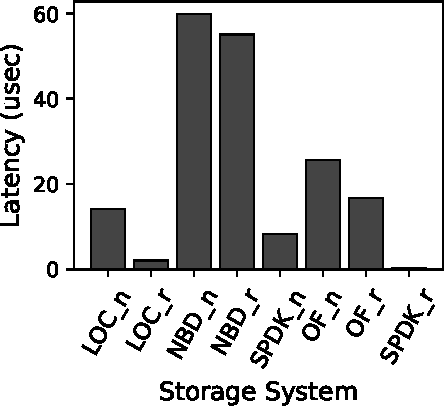
\includegraphics[width=\linewidth]{figures/fio_512.pdf}\\
\caption{Average latency (usec) of local and remote storage systems with 512 B request size. "r" stands for ramdisk and "n" stands for NVMe, "OF" stands for NVMe-oF with SPDK User-Space drivers.}
\label{fig:fio_512}
\end{figure}

We will analyze the results to determine the best setup for evaluating Teraheap. Starting with local SSD FIO reports an average of 14.16 $\mu$s latency and for local ramdisk, FIO reports 2.04 $\mu$s 6.94$\times$ better. First, we will investigate the remote option NBD (TCP). The exported SSD with NBD average latency is 4.22$\times$ higher than local with an average of 59.86 $\mu$s. Meaning that we get 45.7 $\mu$s more latency with NBD. By looking at the Exported ramdisk with NBD average latency is 1.08$\times$ better than the NBD SSD, meaning that there is a common overhead. This overhead can either be the NBD I/O path or high TCP latency. We use Netperf to measure the TCP latency and conduct experiments with 512 bytes of data in each packet. Netperf reports 37.84 $\mu$s average
latency. Adding local NVMe and TCP latency we have 52 $\mu$s 7.86 $\mu$s difference to the NBD
(TCP) latency 59.86 $\mu$s. We conclude that the primary overhead is TCP, accounting for 63.2\% of the average latency in NBD NVMe.

Next, we investigate lowering the latency of the local I/O path to the device by using userspace drivers (SPDK). With userspace drivers, we bypass the layers of the kernel's I/O stack and eliminate context switches. We run FIO on the NVMe with SPDK and get 8.31 $\mu$s average latency 1.7$\times$ better compared to traditional drivers. We also try to lower
the network latency with NVMe-oF NVMe with SPDK User-Space drivers. With the combination of SPDK’s user-space optimizations, the efficient protocol design of NVMe-oF compared to TCP and RDMA with Infiniband transport layer we manage to measure 25.69 $\mu$s average latency 2.33$\times$ better than SSD with NBD. 

Moving on SPDK ramdisk outperforms everything with 0.33 $\mu$s average latency, but the NVMe-oF ramdisk with SPDK User-Space drivers have 16.66 $\mu$s average latency 9.03 $\mu$s better than the NVMe-oF NVMe and only 1.54$\times$ better compared to the local performance where the local ramdisk is 25.18$\times$ better. There is a common overhead in both NVMe-oF setups which is attributed either to the NVMe I/O path or network latency. Previously we measured the NVMe with SPDK User-Space drivers and got 8.31 $\mu$s a logical 32.34\% of the NVMe-oF NVMe with SPDK latency. We used ib\_read\_lat to conduct RDMA Read Latency Test with 512 bytes requests and we measure that the infiniband ports average latency is 2 $\mu$s only 7.78\% of the NVMe-oF NVMe with SPDK latency meaning that the high latency can be by the Linux Kernel NVMe-oF Initiator which uses traditional kernel I/O calls to the exported /dev device and then the calls are encapsulated and transported to the target via infiniband. Unfortunately, SPDK's user-space NVMe-oF initiator doesn't directly create block devices in /dev, SPDK uses its own bdev (block device) layer which will not be
compatible for later experiments with TeraHeap. 

\begin{figure}[H]
  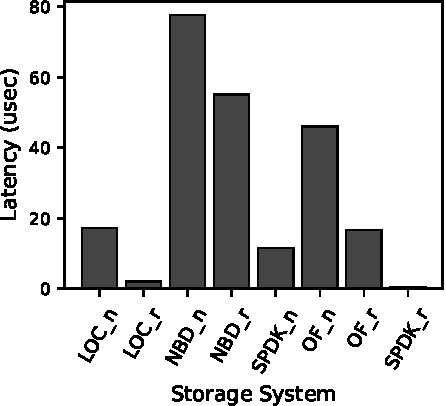
\includegraphics[width=\linewidth]{figures/fio_4k.pdf}\\
\caption{Average latency (usec) of local and remote storage systems with 4KB request size."r" stands for ramdisk and "n" stands for NVMe, "OF" stands for NVMe-oF with SPDK User-Space drivers.}
\label{fig:fio_4k}
\end{figure}

Similarly, with 4KB block size we get the same overheads as shown in figure
\ref{fig:fio_4k}. Here FIO reports more latency for moving the 4KB data locally
and/or across network. The NVMe-oF NVMe with SPDK achieving 25.69 $\mu$s and the NVMe-oF ramdisk with SPDK reaching 16.66 $\mu$s average latency (nearly as fast as the
local NVMe at 14.16 microseconds) are suitable to proceed with our evaluation
using Teraheap.



\subsection{TeraHeap performance with NVMe-oF}
\par This section compares TeraHeap performance of two setups one with local NVMe device and one with NVMe-oF exported NVMe with SPDK User-Space drivers. Figure \ref{fig:bench_spark} illustrates the performance of TeraHeap with Spark workloads for both setups. 
\begin{figure}[H]
  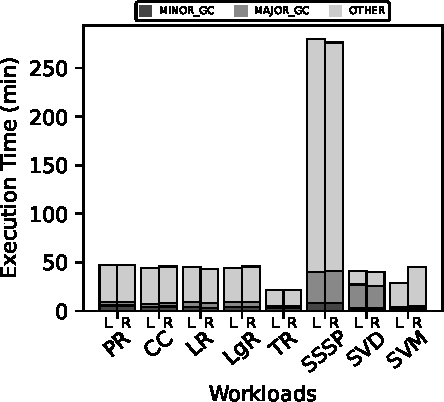
\includegraphics[width=\linewidth]{figures/bench_spark.pdf}\\
\caption{TeraHeap Spark performance. local NVMe device (L) compared to NVMe-oF exported NVMe with SPDK (R).}
\label{fig:bench_spark}
\end{figure}
The two TeraHeap setups local NVMe device (L) and NVMe-oF exported NVMe with SPDK (R) perform similarly with Spark workloads. We can see that the local setup outperforms the remote setup in Pagerank(PR), Connected Components(CC), and Logistic Regression(LgR) making the local setup 0.85\%, 3.55\% and 3.18\% faster accordingly. The big difference is in the SVM workload where the local setup outperforms the remote by 37.30\% \textbf{(why????)}. There are also cases where the remote setup is better. Workloads Linear Regression(LR), Triangle Counts(TR), Shortest Path(SSSP) and SVDPlusPlus(SVD) report that the remote setup is 4.76\%, 2.08\%, 1.37\% and 2.76\% quicker accordingly. Spark Workloads read objects from H2 but don't change them so heavy write operations are missing.

Next, we run Teraheap with the Giraph Workloads. These workloads read objects from H2 and also change them. Here we expect heavy write operations that can stress the remote setup. Figure \ref{fig:bench_giraph} illustrates the performance of TeraHeap with Giraph workloads for both setups NVMe device (L) and NVMe-oF exported NVMe with SPDK (R).
\begin{figure}[H]
  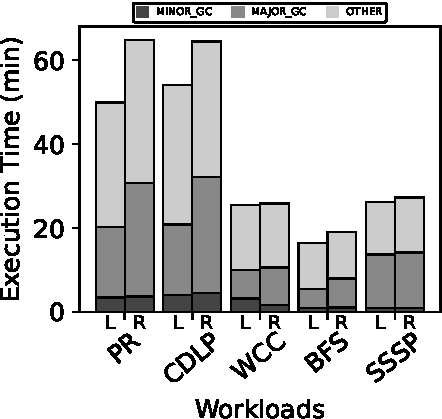
\includegraphics[width=\linewidth]{figures/bench_giraph.pdf}\\
\caption{TeraHeap Giraph performance. local NVMe device (L) compared to NVMe-oF exported NVMe with SPDK (R).}
\label{fig:bench_giraph}
\end{figure}
Here, due to the write operations, the remote setup (R) never manages to exceed the performance of the local setup (L). PageRank (PR), CDLP and BFS workloads are the ones that the remote setup struggles the most here local setup is 22.97\% 16.24\% and 13.07\% quicker accordingly. In the setups mentioned before the remote setup is losing performance due to major GC's taking more time to complete. Following up with WCC and SSSP workloads we can see that the local setup is only 1.54\%	and 3.97\% faster again here major GC's are the reason the remote setup is slower.

\subsection{Workload disk statistics}

 In this section we review the disk statistics of the workload runs. First we examine Spark. figures \ref{fig:spark_r} and \ref{fig:spark_w} show reads and writes accordingly. First we can confirm that reads are more than writes due to the nature of spark benchmarks. Next focusing on the reads we can see that the Gigabytes read for both the local setup (L) and the remote setup (R) are close. An exception here is the SVM workload where the remote setup haves 8.3$\times$ more Gigabytes of reads.
 
 Next we examine Giraph. figures \ref{fig:giraph_r} and \ref{fig:giraph_w} show reads and writes accordingly. Focusing on the writes we can see that the data in Gigabytes for both the local setup (L) and the remote setup (R) are close. In the PageRank(PR)	and CDLP workloads where the local setup (L) haves the best performance compared to the remote setup (R) (figure \ref{fig:bench_giraph} 22.97\% and 16.24\% faster) we can see more reads (figure \ref{fig:giraph_r}) for the remote setup due to more major GC's.

\begin{figure}[H]
  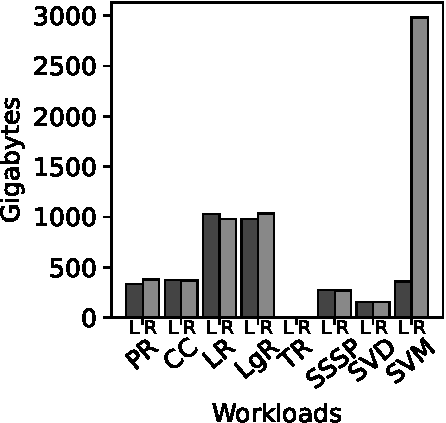
\includegraphics[width=\linewidth]{figures/spark_r.pdf}\\
\caption{Teraheap Spark workloads reads (GB). local NVMe device (L) compared to NVMe-oF exported NVMe with SPDK (R).}
\label{fig:spark_r}
\end{figure}
\begin{figure}[H]
  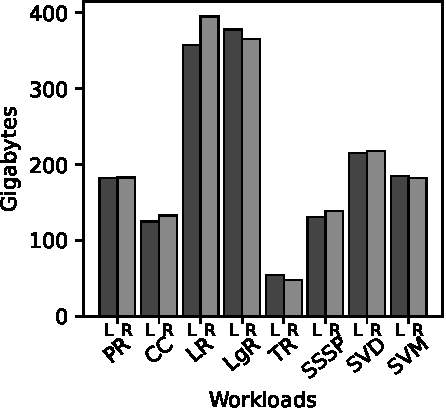
\includegraphics[width=\linewidth]{figures/spark_w.pdf}\\
\caption{Teraheap Spark workloads writes (GB). local NVMe device (L) compared to NVMe-oF exported NVMe with SPDK (R).}
\label{fig:spark_w}
\end{figure}
\vspace{10em}
\begin{figure}[H]
  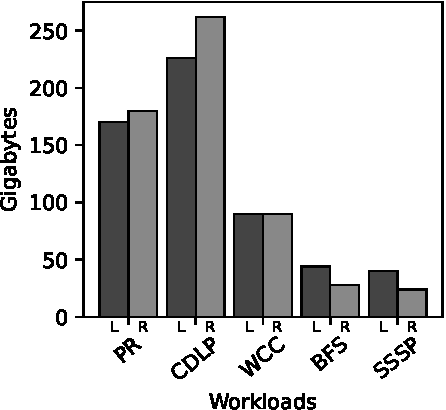
\includegraphics[width=\linewidth]{figures/giraph_r.pdf}\\
\caption{Teraheap Giraph workloads reads (GB). local NVMe device (L) compared to NVMe-oF exported NVMe with SPDK (R).}
\label{fig:giraph_r}
\end{figure}

\begin{figure}[H]
  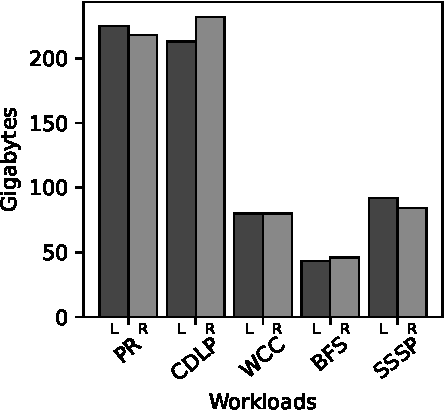
\includegraphics[width=\linewidth]{figures/giraph_w.pdf}\\
\caption{Teraheap Giraph workloads writes (GB). local NVMe device (L) compared to NVMe-oF exported NVMe with SPDK (R).}
\label{fig:giraph_w}
\end{figure}

\section{Conclusions}
Big data analytics frameworks on JVMs are widely used in data centers for large dataset analysis. Research has explored extending the managed heap with fast local storage (e.g., NVMe SSDs) and remote memory, but comprehensive performance and reliability comparisons are lacking. In our comparative analysis, we first employed micro-benchmarks to explore the latency and throughput performance of various storage systems, including local NVMe, remote NVMe, and remote memory. We then selectively compared local device systems with NVMe-oF SPDK NVMe and NVMe-oF SPDK Ram-disk using TeraHeap, which extends the managed heap over these devices. We evaluated these options with 13 widely-used applications in two real-world big data frameworks, Spark and Giraph. The workload reports indicate that NVMe-oF and remote options can match the performance of local ones, yielding very similar results. We found out that the NVMe-oF SPDK NVMe struggles to perform well with the Giraph workloads where there are a lot of writes to objects in the second heap (H2) but the spark workloads have very similar results compared to the local device setup. Finally, we concluded that extending the heap over NVMe-oF SPDK Ram-disk can perform almost the same compared to the local setup in the Giraph workloads. This study provides valuable insights into the performance characteristics of different storage solutions, informing decisions on resource allocation and system design, and contributing to the ongoing discourse on efficient data management in contemporary computing environments.

\bibliographystyle{plain}
\bibliography{paper}

\end{document}

